%% This Beamer template is based on the one found here: https://github.com/sanhacheong/stanford-beamer-presentation, and edited to be used for Stanford ARM Lab

\documentclass[10pt, aspectratio=169]{beamer}
%\mode<presentation>{}

\usepackage{media9}
\usepackage{amssymb,amsmath,amsthm,enumerate}
\usepackage[utf8]{inputenc}
\usepackage{array}
\usepackage[parfill]{parskip}
\usepackage{graphicx}
\usepackage{caption}
\usepackage{subcaption}
\usepackage{bm}
\usepackage{amsfonts,amscd}
\usepackage[]{units}
\usepackage{listings}
\usepackage{multicol}
\usepackage{multirow}
\usepackage{tcolorbox}
\usepackage{physics}
\usepackage{algpseudocode}
\usepackage{mathtools}
\usepackage{algorithmicx, algorithm2e}
\usepackage{ragged2e}

% \usepackage{xcolor}

% Enable colored hyperlinks
\hypersetup{
    colorlinks=true,
    citecolor=uma_pink,
    linkcolor=uma_blue_light,
    filecolor=uma_blue_water,      
    urlcolor=uma_blue_light,
    pdftitle={Overleaf Example},
    pdfpagemode=FullScreen,
}

% Select normal math font
\usefonttheme[onlymath]{serif}

\renewcommand{\thebibliography}{\textcolor{uma_blue_water}{\arabic{bibliography}}}
\renewcommand{\thefigure}{\textcolor{uma_blue_water}{\arabic{figure}}}
\renewcommand{\figurename}{\textcolor{uma_blue_water}{Fig.}}
\renewcommand{\thesubfigure}{\textcolor{uma_blue_water}{\alph{subfigure}}}
\renewcommand{\thetable}{\textcolor{uma_blue_water}{\arabic{table}}}
\renewcommand{\tablename}{\textcolor{uma_blue_water}{Table}}


% The following three lines are for crossmarks & checkmarks
\usepackage{pifont}% http://ctan.org/pkg/pifont
\newcommand{\cmark}{\ding{51}}%
\newcommand{\xmark}{\ding{55}}%

% Numbered captions of tables, pictures, etc.
\setbeamertemplate{caption}[numbered]

%\usepackage[superscript,biblabel]{cite}
\usepackage{algorithm2e}
\renewcommand{\thealgocf}{}

% Bibliography settings
\usepackage[style=ieee]{biblatex}
\setbeamertemplate{bibliography item}{\insertbiblabel}
\addbibresource{references.bib}

% Glossary entries
\usepackage[acronym]{glossaries}
\newacronym{ML}{ML}{machine learning}
\newacronym{HRI}{HRI}{human-robot interactions}
\newacronym{RNN}{RNN}{Recurrent Neural Network}
\newacronym{LSTM}{LSTM}{Long Short-Term Memory}


\theoremstyle{remark}
\newtheorem*{remark}{Remark}
\theoremstyle{definition}

\newcommand{\empy}[1]{{\color{uma_blue_dark}\emph{#1}}}
\newcommand{\empr}[1]{{\color{uma_blue_dark}\emph{#1}}}
\newcommand{\examplebox}[2]{
\begin{tcolorbox}[colframe=uma_blue_dark,colback=uma_gray_light,title=#1]
#2
\end{tcolorbox}}

\usetheme{Uma} 
\def \i  {\item}
\def \ai {\item[] \quad \arrowbullet}
\newcommand \si[1]{\item[] \quad \bulletcolor{#1}}
\def \wi {\item[] \quad $\ \phantom{\Rightarrow}\ $}
\def \bi {\begin{itemize}\item}
\def \ei {\end{itemize}}
\def \be {\begin{equation*}}
\def \ee {\end{equation*}}
\def \bie {$\displaystyle{}
\def \eie {{\ }$}}
\def \bsie {\small$\displaystyle{}
\def \esie {{\ }$}\normalsize\selectfont}
\def \bse {\small\begin{equation*}}
\def \ese {\end{equation*}\normalsize}
\def \bfe {\footnotesize\begin{equation*}}
\def \efe {\end{equation*}\normalsize}
\renewcommand \le[1] {\\ \medskip \lefteqn{\hspace{1cm}#1} \medskip}
\def \bex {\begin{example}}
\def \eex {\end{example}}
\def \bfig {\begin{figure}}
\def \efig {\end{figure}}
\def \btheo {\begin{theorem}}
\def \etheo {\end{theorem}}
\def \bc {\begin{columns}}
\def \ec {\end{columns}}
\def \btab {\begin{tabbing}}
\def \etab {\end{tabbing}\svneg\svneg}
\newcommand \col[1]{\column{#1\linewidth}}
\def\vneg  {\vspace{-5mm}}
\def\lvneg {\vspace{-10mm}}
\def\svneg {\vspace{-2mm}}
\def\tvneg {\vspace{-1mm}}
\def\vpos  {\vspace{5mm}}
\def\lvpos {\vspace{10mm}}
\def\svpos {\vspace{2mm}}
\def\tvpos {\vspace{1mm}}
\def\hneg  {\hspace{-5mm}}
\def\lhneg {\hspace{-10mm}}
\def\shneg {\hspace{-2mm}}
\def\thneg {\hspace{-1mm}}
\def\hpos  {\hspace{5mm}}
\def\lhpos {\hspace{10mm}}
\def\shpos {\hspace{2mm}}

\logo{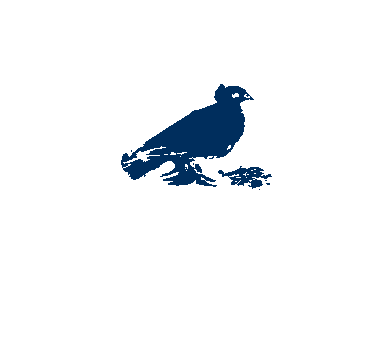
\includegraphics[height=0.8cm]{./style_files_uma/logo_uma_negativo}\hspace{0.1cm}}

% commands to relax beamer and subfig conflicts
% see here: https://tex.stackexchange.com/questions/426088/texlive-pretest-2018-beamer-and-subfig-collide
\makeatletter
\let\@@magyar@captionfix\relax
\makeatother

\title[\href{https://jmgandarias.com}{\textcolor{white}{jmgandarias.com}}]{Trajectory Planning in the Operational Space}

%\subtitle{Subtitle Of Presentation}

%\beamertemplatenavigationsymbolsempty

\begin{document}
\justifying

\author[Systems Engineering and Automation]{
	\large
	Juan M. Gandarias\\
    \footnotesize \href{mailto:jmgandarias@uma.es}{jmgandarias@uma.es}
}

\institute{
	\textcolor{uma_gray_dark}{
    Systems Engineering and Automation Department\\
	University of Malaga\\
    \href{https://www.uma.es/imech/}{IMECH.UMA}}
 	\vskip 5pt
    % \small{\date{\today}}
 %    \begin{figure}
	% 	\centering
	% 	\begin{subfigure}[t]{0.5\textwidth}
	% 		\centering
	% 		
\includegraphics[height=1.5cm]{./style_files_uma/logo_uma}
	% 	\end{subfigure}%
	% 	~
	% 	\begin{subfigure}[t]{0.5\textwidth}
	% 		\centering
	% 		\includegraphics[height=0.33in]{./images/arm_lab_logo_with_title_small_adj_6.png}
	% 	\end{subfigure}
	% \end{figure}
}


\date{\today}

\begin{noheadline}
\begin{frame}
    \maketitle
    \vspace{-1cm}
    \begin{figure}
		\centering
		
\includegraphics[height=1.5cm]{./style_files_uma/logo_uma}
        \hspace{10cm}
        
\includegraphics[height=1.4cm]{./style_files_uma/logo_isa}
	\end{figure}
 %    \begin{figure}
	% 	\centering
	% 	\begin{subfigure}[t]{0.5\textwidth}
	% 		\centering
	% 		
\includegraphics[height=1.5cm]{./style_files_uma/logo_uma}
	% 	\end{subfigure}%
	% 	~
	% 	\begin{subfigure}[t]{0.5\textwidth}
	% 		\centering
	% 		\includegraphics[height=0.33in]{./images/arm_lab_logo_with_title_small_adj_6.png}
	% 	\end{subfigure}
	% \end{figure}
 \end{frame}
\end{noheadline}



\setbeamertemplate{itemize items}[circle]
% \setbeamertemplate{itemize subitem}[square]

\begin{frame}
	\frametitle{Outline} % Table of contents slide, comment this block out to remove it
	\tableofcontents % Throughout your presentation, if you choose to use \section{} and \subsection{} commands, these will automatically be printed on this slide as an overview of your presentation
\end{frame}



\section{Introduction}

\begin{frame}
	\frametitle{Outline} % Table of contents slide, comment this block out to remove it
	\tableofcontents[currentsection] % Throughout your presentation, if you choose to use \section{} and \subsection{} commands, these will automatically be printed on this slide as an overview of your presentation
\end{frame}

\begin{frame}[allowframebreaks]
\frametitle{Introduction}
	\begin{itemize}
    
	    \item \textbf{Trajectory Planning:} To generate the references to the motion control system of a robotic manipulator.
        \begin{itemize}
            \item References are computed from a polynomial that adjusts to the desired trajectory.
            \item During the whole motion from the initial to the last pose the actuators are not saturated (smooth trajectories).
        \end{itemize}
        
    \item \textbf{Path:} Sequence of points in the joint or operational (Cartesian) space. 
    
    \item \textbf{Trajectory:} Path with a temporal law in terms of velocity or acceleration (path + schedule) \cite{paths_and_trajectories}.
    
    \item \textbf{Joint space:} Set of all possible positions and orientations of a robot's joints (a.k.a. configuration space).
    
    $\mathbf{q} = [q_1, ..., q_n ]^T \in \mathbb{R}^n$, $n \equiv \textrm{number of joint DoFs}$ 

    \framebreak
    
    \item \textbf{Operational space:} Space in which the robot's end-effector operates. Defined by the EE pose (a.k.a. task space).

    \item \textbf{Cartesian space:} Operational space described by the Cartesian coordinates and orientation angles.
    
    $\mathbf{x} = [\underbrace{x, y, z}_{position}, \underbrace{\alpha_x, \alpha_y, \alpha_z}_{orientation}] \in \mathbb{R}^6$.

    \item \textbf{Kinematics:} Study of motion without forces

    \begin{itemize}
        \item Forward kinematics: $\mathbf{x} = f(\mathbf{q})$
        \item Inverse kinematics: $\mathbf{q} = g(\mathbf{x})$
        \item First-order differential kinematics (Jacobian): $\mathbf{\dot{x}} = \mathbf{J}(\mathbf{q}) \cdot \mathbf{\dot{q}}$, \hspace{0.2cm} $\mathbf{\dot{q}} = \mathbf{J}^{-1}(\mathbf{q}) \cdot \mathbf{\dot{x}}$
    \end{itemize}
    
	\end{itemize}

    \framebreak

    \begin{center}
    \begin{minipage}{.45\linewidth}
    \begin{figure}
            \centering
            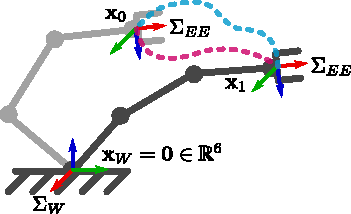
\includegraphics{images/manipulator_path.pdf}
            \caption{Cartesian paths illustration.}
    \end{figure}
    \end{minipage}%
    \begin{minipage}{.6\linewidth}
    \begin{itemize}
        \item $\mathbf{x}_0$ and $\mathbf{x}_1$ are EE poses w.r.t. $\mathbf{\Sigma}_W$
        \item Thanks to inverse kinematics, we can calculate $\mathbf{q}_1 = g(\mathbf{x}_1)$ 
        \item If we set this value to the motors, the robot will move towards that pose
        \item But...
        \begin{itemize}
            \item Which path will be followed?
            \item Which trajectory? 
            \item How can we control it? $\rightarrow$ Trajectory Planning
        \end{itemize}
    \end{itemize}
    \end{minipage}
    \end{center}

    \framebreak
    \begin{itemize}
        \item If there is an obstacle in the way of the robot, or if we want the robot to keep a specific orientation over the path (e.g., it carries a glass of water) $\Rightarrow$ \textcolor{uma_pink}{WE NEED A TRAJECTORY}
        \item \textbf{Generating the path:} Calculate a set of intermediate pose references (waypoints).
        \item \textbf{Generating the trajectory:} 
        \begin{enumerate}
            \item Set the arrival times to each of these waypoints.
            \item Define the polynomial to ensure a smooth trajectory.
        \end{enumerate}

        \vspace{0.5cm}
        \begin{figure}
            \centering
            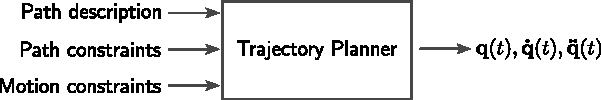
\includegraphics{images/trajectory_planner_schema.pdf}
            \caption{Trajectory planner diagram.}
            % \caption{Cartesian paths illustration.}
        \end{figure}
        
    \end{itemize}

    \framebreak
    Two trajectory Planning approaches:
    
    \begin{center}
    \begin{minipage}[t]{.5\linewidth}
        \textbf{\textcolor{uma_blue_dark}{Trajectories in the Joint Space:}}
        \begin{itemize}
            \item Planning in terms of controlled variables $(\mathbf{q}(t))$.
            \item A polynomial is generated for each joint.
            \item Lightweight computation.
            \item Easy to compute in real-time.
            \item Hard to determine the actual Cartesian motion.
            \item The EE trajectory is not controllable.
        \end{itemize}
    \end{minipage}
    \begin{minipage}[t]{.49\linewidth}
        \textbf{\textcolor{uma_blue_dark}{Trajectories in the Operational Space:}}
        \begin{itemize}
            \item Essential for tasks in the operational space.
            \item The EE Cartesian trajectory is known.
            \item Need to compute inverse kinematics (including $\mathbf{J}^{-1}$).
            \item Higher computational cost.
            \item Have to deal with singularities.
            \item The orientation is not unique.
            
        \end{itemize}
    \end{minipage}
    \end{center}

  
\end{frame}

\section{Trajectory Planning in the Joint Space}
\begin{frame}
	\frametitle{Outline} % Table of contents slide, comment this block out to remove it
	\tableofcontents[currentsection] % Throughout your presentation, if you choose to use \section{} and \subsection{} commands, these will automatically be printed on this slide as an overview of your presentation
\end{frame}


\begin{frame}[allowframebreaks]
\frametitle{Trajectory Planning in the Joint Space}

\textbf{\textcolor{uma_blue_dark}{Algorithm}}

\begin{minipage}[T!]{.48\linewidth}
\begin{algorithm}[H]
	$\mathbf{X} \gets \textsf{Knots}$\;
    $\mathbf{Q} = \textsf{inverse\_kinematics}(\mathbf{X})$\;
    $\mathcal{H}(t) \gets \mathcal{J}(\mathbf{Q}, t_f)$\;
    $t_k = 0$\;
	\While{$t_k < t_f$}
 	{
        $t_k = t_k + \Delta t$\;
        $\mathbf{q}_{d} = \mathcal{H}(t_k)$\;
        publish($\mathbf{q}_{d}$)\;
        sleep($\Delta t$);
  	}
\end{algorithm}
\end{minipage}
\begin{minipage}[T!]{.42\linewidth}
\begin{itemize}
    \item $\mathbf{X} = [\mathbf{x}_0, \dots, \mathbf{x}_l]\in\mathbb{R}^{6 \times l}$
    \item $\mathbf{Q} = [\mathbf{q}_0, \dots, \mathbf{q}_l]\in\mathbb{R}^{n \times l}$
    \item $\mathcal{J}\equiv$ polynomial interpolation.
    \item $l \equiv$ number of locations (knots).
    \item $t_k \equiv$ time at step $k$.
    \item $t_f \equiv$ final time.
    \item We get a trajectory for each joint (by interpolation).
    \item Not a Cartesian trajectory.
\end{itemize}
\end{minipage}

Different types of $\boldsymbol{h}(\mathbf{Q}, t_f)$ (already studied in Robot Programming and Control)~\cite{joint_trajectory_planning}:
\begin{itemize}
    \item Cubic polynomials, Quintic polynomials, Linear Segments with Parabolic Blends (LSPB)~\cite{point_to_point}.
\end{itemize}


\end{frame}

\section{Trajectory Planning in the Cartesian Space}
\begin{frame}
	\frametitle{Outline} % Table of contents slide, comment this block out to remove it
	\tableofcontents[currentsection] % Throughout your presentation, if you choose to use \section{} and \subsection{} commands, these will automatically be printed on this slide as an overview of your presentation
\end{frame}

\begin{frame}[allowframebreaks]
\frametitle{Trajectory Planning in the Operational Space}

\begin{itemize}
    \item We must schedule the Cartesian locations (poses) of the EE between the initial and final poses~\cite{cartesian_trajectory_planning}.
    \item The polynomial interpolation is conducted in the Operational Space (Cartesian interpolation):
    
    $
    \mathbf{h}(t_k) = \textsf{cartesian\_interpolation}(\mathbf{x}, t_f)\in\mathbb{R}^6
    $
    
    \item Position and Orientation along the generated Cartesian path must be defined separately (different representations).
    \item High actuators control frequency $\rightarrow$ real-time.
    \item The number of Cartesian locations (knots) to be interpolated in the Cartesian space is typically low (2 knots for point-to-point, 2 knots if using a via point).
    \item Simple interpolating paths in the Cartesian space (e.g., straight lines, arc of circles). Not necessary simple in the joint space.
\end{itemize}

\framebreak

\textbf{\textcolor{uma_blue_dark}{Algorithm}}

\begin{minipage}[T!]{.47\linewidth}
\begin{algorithm}[H]
	$\mathbf{X} \gets \textsf{Knots}$\;
    $\mathcal{H}(t) \gets \mathcal{C}(\mathbf{X}, t_f)$\;
    $t_k = 0$\;
	\While{$t_k < t_f$}
 	{
        $t_k = t_k + \Delta t$\;
        $\mathbf{x}_d = \mathcal{H}(t_k)$\;
        $\mathbf{q}_{d} =  \textsf{inverse\_kinematics}(\mathbf{x}_d)$\;
        publish($\mathbf{q}_{d}$)\;
        sleep($\Delta t$);
  	}
\end{algorithm}
\end{minipage}
\begin{minipage}[T!]{.42\linewidth}
\begin{itemize}
    \item $\mathcal{C}\equiv$ Cartesian interpolation.
    \item $l \equiv$ number of locations (knots).
    \item We get the Cartesian trajectory (by interpolation).
    \item We command the desired $\mathbf{q}_{d}$ obtained from kinematics inversion.
\end{itemize}
\end{minipage}
\end{frame}

% \begin{frame}[allowframebreaks]
% \frametitle{Methods for Cartesian Trajectory Planning}
% \begin{enumerate}
%     \item Bounded deviation joint paths.

%     \item Cartesian interpolation.
    
%     \begin{enumerate}
%         \item Homogeneous matrix interpolation.
%         \item Position interpolation
%         \item Orientation interpolation
%         \item Quaternions interpolation.
%         \item Smooth Cartesian trajectory planning.
%     \end{enumerate}
    

%     \item Optimal trajectory planning.
%     \begin{enumerate}
%         \item Dynamic scaling of the trajectories.
%     \end{enumerate}

%     % \item Optimal trajectory planning~\cite{vukobratovic1982method}.
% \end{enumerate}
% \end{frame}

\section{Bounded Deviation Joint Paths}
\begin{frame}
	\frametitle{Outline} % Table of contents slide, comment this block out to remove it
	\tableofcontents[currentsection] % Throughout your presentation, if you choose to use \section{} and \subsection{} commands, these will automatically be printed on this slide as an overview of your presentation
\end{frame}
\begin{frame}[allowframebreaks]
\frametitle{Bounded Deviation Joint Paths}

A hybrid Cartesian-joint approach: To follow a specific trajectory in the Cartesian space, one could define a series of via points (knots) and plan in the joint space.

A bounded deviation joint path defines enough knots to guarantee that the error (in Cartesian space) is bounded between admissible limits~\cite{taylor1979planning}.

 \begin{center}
    \begin{minipage}{.5\linewidth}
    \begin{figure}
        \centering
        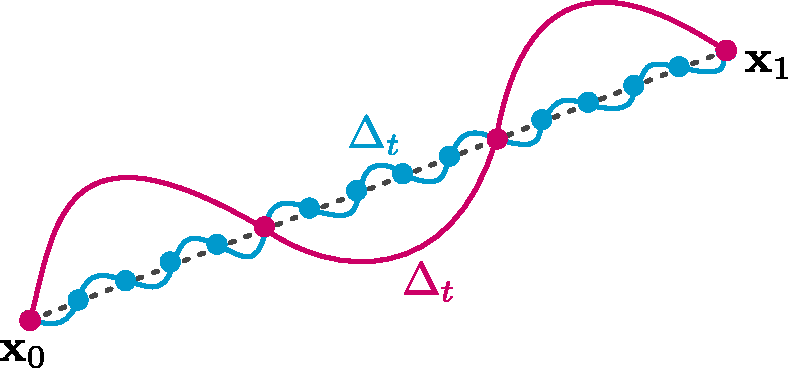
\includegraphics[width = 0.8\textwidth]{images/bounded_joint_path.pdf}
        \caption{Bounded deviation paths.}
    \end{figure}
    
    \begin{footnotesize}
        $\cdots$ Desired Cartesian path.
    
        \textcolor{uma_pink}{$-$ Bounded deviation path with few knots.}
    
        \textcolor{uma_blue_light}{$-$ Bounded deviation path with many knots.}    
    \end{footnotesize}
    
    \end{minipage}%
    \hspace{0.5cm}
    \begin{minipage}{.45\linewidth}
    \textcolor{uma_pink}{\textbf{Low number of knots:}}
        \begin{itemize}
            \item Low computation.
            \item High $\Delta_t$.
            \item High error.
        \end{itemize}
    \textcolor{uma_blue_light}{\textbf{High number of knots:}}
    \begin{itemize}
        \item High computation.
        \item Low $\Delta_t$.
        \item Low error.
    \end{itemize}
    \end{minipage}
\end{center}

    \framebreak

    \textbf{\textcolor{uma_blue_dark}{Recursive pre-planning method}}

    First, define the maximum position and orientation errors:
    $
    \delta_p^{\textsf{max}} = |p_j(t)-p_{j-1}(t-1)|, \, \delta_r^{\textsf{max}} = |\varphi|
    $
    \begin{enumerate}
        \item Calculate $\mathbf{q}_0$ and $\mathbf{q}_1$ (Inverse Kinematics).
        \item Compute the intermediate joint configuration $\mathbf{q}_i = \mathbf{q}_1-\frac{1}{2}\Delta\mathbf{q}_0$.
        \item Compute the intermediate Cartesian configuration $\mathbf{x}_i = \textsf{Forward Kinematics}(\mathbf{q}_i)$.
        \item Compute the bounded errors $\delta_p$ and $\delta_r$.
        \item Check the bounded errors $\delta_p \leq \delta_p^{\textsf{max}} $ and $\delta_r \leq \delta_r^{\textsf{max}}$.
        \item If the conditions are not satisfied, repeat steps 2 to 5 for the new segments created.
    \end{enumerate}

    Higher errors usually appear at the beginning and end of the trajectories (due to high velocity changes).
    


\end{frame}

\section{Cartesian Interpolation}
\subsection{Homogeneous Matrix Interpolation}
\begin{frame}
	\frametitle{Outline} % Table of contents slide, comment this block out to remove it
	\tableofcontents[currentsection,
        currentsubsection] % Throughout your presentation, if you choose to use \section{} and \subsection{} commands, these will automatically be printed on this slide as an overview of your presentation
\end{frame}

\begin{frame}[allowframebreaks]
\frametitle{Homogeneous Matrix Interpolation}

This method was proposed by Richard Paul~\cite{paul1979manipulator} in 1975 in an International Conference (although formally published in a scientific journal in 1979) to make up paths consist of straight line segments connected by smooth transitions with controlled acceleration.

\textcolor{uma_blue_dark}{\textbf{Concept}}
\begin{itemize}
    \item One of the simplest ways to change from one transform to the other is by a straight line translation and a rotation about same fixed axis in space.
    \item With such a line and axis then we can produce a motion of controlled linear and angular velocity.
    \item  However, the motion is made in terms of a translation and two rotations. The first rotation will serve to align the tool in the required final direction and the second rotation will control the orientation of the tool about the tool axis.
    \item As all manipulators end in a rotary joint, this second rotation in space corresponds to a rotation of the final joint of the manipulator. 
\end{itemize}

\framebreak


\begin{center}
    \begin{minipage}{.45\linewidth}
        \begin{figure}
            \centering
            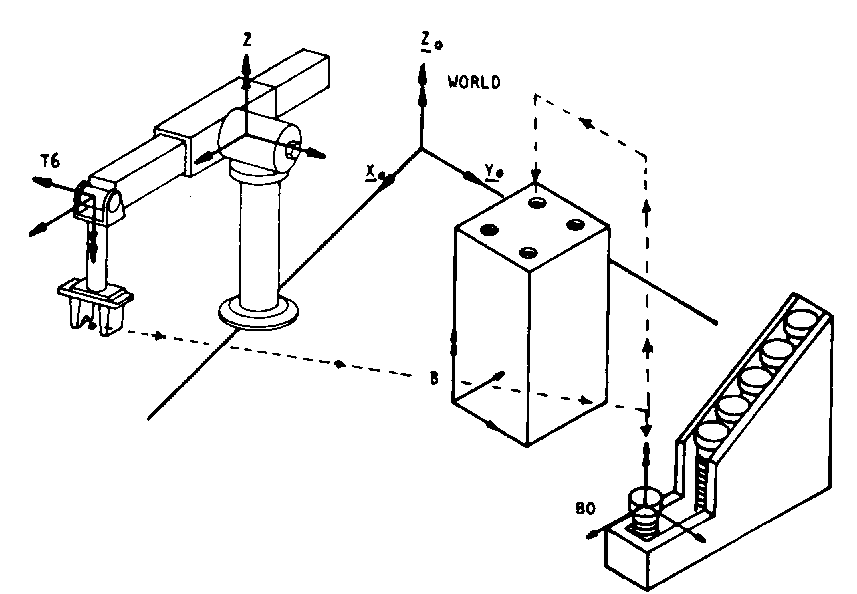
\includegraphics[width = 1\textwidth]{images/industrial_manipulator_task.pdf}
            \caption{Typical industrial manipulation task (source:~\cite{luh1983conventional}).}
        \end{figure}
    \end{minipage}%
    \hspace{0.5cm}
    \begin{minipage}{.5\linewidth}
    3 basic motions
    \begin{itemize}
        \item Translation: Linear displacement from $\mathbf{x}_A$ to $\mathbf{x}_B$.
        \item Rotation around translation axis: Ensuring Z-axis fo the EE and Z-axis of $\mathbf{x}_B$ are coincident.
        \item Rotation around Z-axis: Orient the EE (tool).  
    \end{itemize}
    \end{minipage}
\end{center}

\framebreak

\begin{figure}
    \centering
    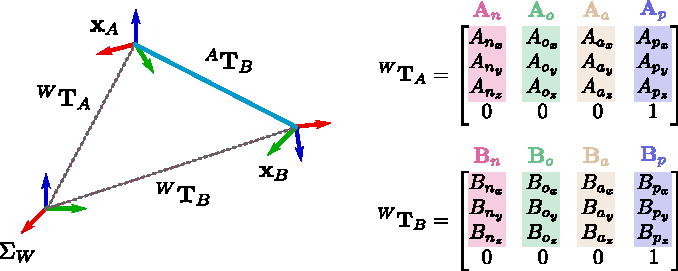
\includegraphics[width = 0.8\textwidth]{images/linear_segment.pdf}
    \caption{Linear segment representation between positions following the nomenclature in~\cite{paul1979manipulator}.}
\end{figure}

\framebreak

The homogeneous transformation between points $A$ and $B$ w.r.t. the world frame $W$ is defined as
$$
^A\mathbf{T}_B = \begin{bmatrix}
    \mathbf{A}_n\mathbf{B}_n & \mathbf{A}_n\mathbf{B}_o & \mathbf{A}n\mathbf{B}_a & \mathbf{A}_{n}(\mathbf{B}_p - \mathbf{A}_p) \\
    \mathbf{A}_o\mathbf{B}_n & \mathbf{A}_o\mathbf{B}_o & \mathbf{A}o\mathbf{B}_a & \mathbf{A}_{o}(\mathbf{B}_p - \mathbf{A}_p) \\
    \mathbf{A}_a\mathbf{B}_n & \mathbf{A}_a\mathbf{B}_o & \mathbf{A}a\mathbf{B}_a & \mathbf{A}_{a}(\mathbf{B}_p - \mathbf{A}_p) \\
    0 & 0 & 0 & 1 \\
\end{bmatrix}
$$
This transformation is the result of applying the three motions described above (one translation $\mathbf{T}$ and two rotations $\mathbf{R}_a$ and $\mathbf{R}_b$)
$$
^A\mathbf{T}_B = \mathbf{T} \cdot \mathbf{R}_a \cdot\mathbf{R}_b
$$

To achieve a desired Cartesian path, We can choose intermediate values of $^A\mathbf{T}_B $ representing a translation and two rotations. To achieve a linear segment (linear interpolation) we will choose intermediate values $h$ of $^A\mathbf{T}_B$, where $h\in\mathbb{R} : 0\leq h \leq 1$. 

\framebreak

The translation will be along the line joining $A$ and $B$ and will be represented by the transformation $T(h)$. The first rotation will serve to rotate the approach vector, the direction in which the tool is pointing, from $A$ into the approach vector at $B$. This rotation will be represented by $R_a(h)$. The second rotation will rotate the orientation vector, representing the orientation of the tool, from $A$ into the orientation vector at $B$, $R_o(h)$. We will then represent $^A\mathbf{T}_B(h)$ as
$$
^A\mathbf{T}_B(h) = \mathbf{T}(h) \cdot \mathbf{R}_a(h) \cdot \mathbf{R}_b(h)
$$

Then, if $h=0 \implies ^A\mathbf{T}_B(0) = ^W\mathbf{T}_A$ and $h=1 \implies ^A\mathbf{T}_B(1) = ^W\mathbf{T}_B$.



\framebreak 

This way, varying $h$ linearly over time, the EE of the manipulator will follow a perfect linear trajectory in the Cartesian space.

According to this, both the translation and rotations will be directly proportional to $h$ so that if $h$ varies linearly with respect to time,  the motion represented by $^A\mathbf{T}_B(h)$ will correspond to a constant linear and two constant angular velocities. 

However, this approach presents some drawbacks:

\begin{itemize}
    \item The rotation is performed in two steps, offering a solution that is unnecessarily complex.
    \item The translation is uniform, but the rotation is not.
    \item The composition of two rotations will usually produce some undesired angular accelerations and requires the computation of rotations around two axes.
\end{itemize}
 
\end{frame}

\subsection{Interpolation of the Position}
\begin{frame}
	\frametitle{Outline} % Table of contents slide, comment this block out to remove it
	\tableofcontents[currentsection,
        currentsubsection] % Throughout your presentation, if you choose to use \section{} and \subsection{} commands, these will automatically be printed on this slide as an overview of your presentation
\end{frame}
\begin{frame}[allowframebreaks]
\frametitle{Interpolation of the Position}

The method proposed by Russel H. Taylor~\cite{taylor1979planning} in 1979 is more convenient (specially for the orientation, as we will see later). 

\begin{itemize}
    \item In that same paper, he also proposed the Bounded Deviation Joint Path method claiming that it is more suitable for real-time control as it requires less computational load. 
    \item While this is true (and especially relevant given the context and time in which that paper was published - the computational capabilities of the hardware we have now are much better than they were in 1979), in this course we are more focused on an accurate solution for Cartesian path planning, rather than a computationally inexpensive solution.
\end{itemize}

\framebreak

To move the EE in a straight path from $\mathbf{p}_0$ to $\mathbf{p}_1$ in time $T$, Taylor proposed a time law according to
$$
\lambda (t) = \frac{T-t}{T}, \quad  \lambda\in[0,1]
$$

where $t$ is the actual time, and $T$ is the final time of the trajectory. 

Hence, the linearly interpolated translation was defined by:
$$
\mathbf{p} (t) = \mathbf{p}_1 - \lambda (t) (\mathbf{p}_1 - \mathbf{p}_0), \quad \mathbf{p}_0, \mathbf{p}_1 \in \mathbb{R}^3
$$

According to this time law, at $\lambda = 0$ the EE is in $\mathbf{p}_1$, and when $\lambda = 1$ the EE is in $\mathbf{p}_0$.

\framebreak

Following this approach we can define \textcolor{uma_pink}{a more suitable time law} that also considers the initial time may be different to 0 as 
\begin{equation}
\lambda (t) = \frac{t-t_i}{t_f-t_i}, \quad  \lambda\in[0,1]
\label{eq:lambda}
\end{equation}

where $t$ is the actual time, and $t_f$ and $t_i$ are the final and initial time of the trajectory. 

Hence, the linearly interpolated translation was defined by:
\begin{equation}
\mathbf{p} (t) = \mathbf{p}_0 + \lambda (t) (\mathbf{p}_1 - \mathbf{p}_0)
\label{eq:p_inter}
\end{equation}

\textcolor{uma_pink}{Note that this equation has now changed compared to the one in the previous slide!}

According to this time law, at $\lambda = 0$ the EE is in $\mathbf{p}_0$, and when $\lambda = 1$ the EE is in $\mathbf{p}_1$.


\end{frame}



\subsection{Interpolation of the Orientation}
\begin{frame}
	\frametitle{Outline} % Table of contents slide, comment this block out to remove it
	\tableofcontents[currentsection,
        currentsubsection] % Throughout your presentation, if you choose to use \section{} and \subsection{} commands, these will automatically be printed on this slide as an overview of your presentation
\end{frame}
\begin{frame}[allowframebreaks]
\frametitle{Interpolation of the Orientation}

Orientation does not have a unique representation. Hence, when we interpolate the orientation, the outcome trajectory is different depending on which representation are we using.

This is due to the following reasons

\begin{itemize}
    \item \textbf{Non-linearity:} The space of rotations is non-linear, and different representations handle this non-linearity in different ways. 
    \item \textbf{Singularities:} Some representations, like Euler angles, have singularities (e.g., gimbal lock) that can cause abrupt changes in the interpolated trajectory.
    \item \textbf{Mathematical Properties:} Some representations have properties that make them more suitable for interpolation. 
\end{itemize}

\framebreak

\begin{enumerate}
    \item \textbf{Rotation matrix}
    \begin{itemize}
        \item \textit{Description:} A $3 \times 3$ matrix that represents rotation in 3D space.
        \item \textit{Interpolation:} Interpolating rotation matrices directly is not straightforward. Intermediate matrices may not be orthonormal, i.e., not rotation matrices (they MUST be orthonormal).

        Example~\cite{barrientos2007fundamentos}: Given $R_i$ and $R_f$
        $$
        \mathbf{R}_i = \begin{bmatrix}
        1 & 0 & 0 \\
        0 & 1 & 0 \\
        0 & 0 & 1
        \end{bmatrix}
        \quad
        \mathbf{R}_f = \begin{bmatrix}
        0 & -1 & 0 \\
        0 & 0 & -1 \\
        1 & 0 & 0
        \end{bmatrix}
        $$
        An element-by-element linear interpolation will result in the intermediate matrix 
        $$
        \mathbf{R}_m = \begin{bmatrix}
        1/2 & -1/2 & 0 \\
        0 & 1/2 & -1/2 \\
        1/2 & 0 & 1/2
        \end{bmatrix}
        $$
        This is not orthonormal, then $\mathbf{R}_m$ does not represent a valid orientation for the EE.
    \end{itemize}

    \framebreak
    
    \item \textbf{Euler angles}
    \begin{itemize}
        \item \textit{Description:} Euler angles represent orientation using three angles, typically denoted as roll, pitch, and yaw.
        
        \item \textit{Interpolation:} Linear interpolation of Euler angles can be conducted. Considering the initial and final orientations as $(\phi_i, \theta_i, \psi_i)$ and  $(\phi_f, \theta_f, \psi_f)$, respectively, the linear interpolation is given by:
        \begin{equation*}
            \begin{split}
            \phi(t) & = \phi_i + \lambda(t) (\phi_f-\phi_i)\\
            \theta(t) & = \theta_i + \lambda(t) (\theta_f-\theta_i)\\
            \psi(t) & = \psi_i + \lambda(t) (\psi_f-\psi_i)
            \end{split}
        \end{equation*}
        
        This lead to 3 rotations along 3 different axes. The result is a non-intuitive trajectory that can lead to issues like gimbal lock and non-smooth transitions, as the angles are not always independent of each others. Also, applying interpolation with Euler angles to the EE of the robot can result to undesired joint configurations making impossible to arrive to the desired orientation \href{https://eii.cv.uma.es/mod/resource/view.php?id=588131}{[Video showing the issue]}
    \end{itemize}

    \framebreak
    
    \item \textbf{Axis-angle} (a.k.a. rotation vector)~\cite{cartesian_trajectory_planning, lynch2017modern}
    \begin{itemize}
        \item  \textit{Description:} This representation uses a unit vector (axis) and an angle to describe the rotation.
        \begin{equation*}
            \begin{split}
            \mathbf{k}\in\mathbf{R}^3 & \equiv \textsf{unit vector that defines the direction of the rotation axis (Euler axis)}\\
            \theta & \equiv \textsf{Rotation angle over } \mathbf{k}
            \end{split}
        \end{equation*}

        \item Interpolation: We get $\mathbf{k}$ and $\theta$ from $\mathbf{R}_A$ and $\mathbf{R}_B$: $\mathbf{R}(\mathbf{k},\theta) = \mathbf{R}_A^T \cdot \mathbf{R}_B$.

        Then, we interpolate the angle with the temporal law $\theta(t) = \lambda(t) \theta$

        $\forall t \in [t_i, t_f], \quad \mathbf{R}_A \cdot \mathbf{R}(\mathbf{k},\theta(t))$ defines the EE orientation at time $t$.

        However, calculating and interpolating the axis and angle separately can be complex, working with quaternions for interpolation is a common approach.
    \end{itemize}

    \framebreak
    
    \item \textbf{Quaternions}
    \begin{itemize}
        \item \textit{Description:} A quaternion is a 4D complex number system that can represent rotations.

        \textcolor{uma_blue_light}{Why do we want to work with quaternions?}
        
        Because they allow us to represent rotations in 3D and take advantage of complex number operations, allowing for smooth and consistent interpolation of 3D rotations.

        \textcolor{uma_blue_light}{Rotations with complex numbers}

        \begin{itemize}
            \item 2D Rotations

            In 2D a rotation can be represented as a complex number formed by a real number and an imaginary number: $x+yi = [x,y] \rightarrow$ unit vector.

            By representing a 2D rotation in the complex plane we can easily relate the rotation angle with the complex number representation:

            \framebreak

            \begin{center}
            \begin{minipage}{.45\linewidth}
                \begin{figure}
                \hspace{-1.5cm}
                        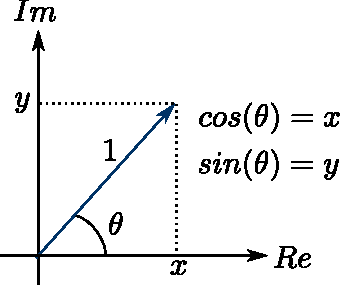
\includegraphics[width = 0.6\textwidth]{images/2D_rotation_complex.pdf}
                        \caption{2D rotation in the complex plane.}
                \end{figure}
                \end{minipage}%
                \begin{minipage}{.5\linewidth}
                    The vector resulting of applying a rotation of $\theta$ is given by the right-hand rule and can be represented with complex numbers as:
                    $$
                    cos (\theta) + sin (\theta) i = [cos(\theta), sin(\theta)]
                    $$
            \end{minipage}
            \end{center}

            Complex numbers multiplication:
            $$
            (x_1+y_1 i)(x_2+y_2 i) = x_1 x_2 - y_1 y_2 + (x_1 y_2 + x_2 y_2)i
            $$

            \framebreak

            \item 3D Rotations

            In 2D we needed 2 elements to represent rotations (a real and an imaginary number).
            In 3D, we need 4 elements: A real and 3 imaginary numbers $\rightarrow$ quaternion~\cite{visualizing_quaternions}

            $$
            \mathbf{q} = \underbrace{w}_{\textsf{real (scalar)}} + \underbrace{xi + yj + zk}_{\textsf{imaginary (vector)}} = [w, x, y, z] = [x, y, z, w] \quad \textsf{\textcolor{uma_pink}{Both notations are allowed!}}
            $$

            \textcolor{uma_pink}{When represented in vectorial format, some people put the real part at the begining and some other at the end. There is no a dominant notation $\rightarrow$ always double-check!}

            \framebreak
            
            A quaternion can be also represented as a rotation of an angle $\theta$ over an axis $\mathbf{n}$ (axis-angle representation) as

            $$
            \textsf{Rot}(\mathbf{n}, \theta) = \left[\underbrace{cos\left(\frac{\theta}{2}\right)}_{w} + \underbrace{sin\left(\frac{\theta}{2}\right) \mathbf{n}}_{\mathbf{v}}\right], \quad \mathbf{n}\in i\mathbb{R}^3
            $$

            $$
            \mathbf{q} = [w, \mathbf{v}], \quad w\in\mathbb{R}, \quad \mathbf{v}\in i \mathbb{R}^3
            $$

            $$
            w = cos\left(\theta/2\right), \quad \mathbf{v} = sin\left(\theta/2\right)\mathbf{n}
            $$

            \begin{equation}
                \theta = 2 acos\left(w\right), \quad \mathbf{n} = \frac{\mathbf{v}}{sin\left(\theta/2\right)}
                \label{eq:axis-angle-quaternion}
            \end{equation}
            
            \framebreak

            Quaternions multiplication:

            \begin{equation*}
                \begin{split}
                    \mathbf{q}_1 \cdot \mathbf{q}_2 & = (w_1+x_1i+y_1j+z_1k)(w_2+x_2i+y_2j+z_2k) = \\
                                             & = (w_1w_2 - x_1x_2 - y_1y_2 - z_1z_2)+ \\
                                             & + (w_1x_2 + x_1w_2 + y_1z_2 - z_1y_2) i +\\
                                             & + (w_1y_2 - x_1z_2 + y_1w_2 + z_1x_2) j +\\
                                             & + (w_1z_2 + x_1y_2 - y_1x_2 - z_1w_2) k\\
                \end{split}
            \end{equation*}

            \begin{equation*}
                \begin{split}
                    & \mathbf{q}_1 = s_1 + \mathbf{v}_1, \quad \mathbf{q}_2 = s_2 + \mathbf{v}_2\\
                    & \mathbf{q}_1 \mathbf{q}_2 = s_1s_2 - \mathbf{v}_1 \cdot \mathbf{v}_2 + s1\mathbf{v}_2 + s_2\mathbf{v}_1 + \mathbf{v}_1 \times \mathbf{v}_2
                \end{split}
            \end{equation*}

            \framebreak

            Relation between quaternions and rotation matrices~\cite{3D_rotation_converter, rotation_calculator}
            $$
            \mathbf{R} = \begin{bmatrix}
                r_{11} & r_{12} & r_{13}\\
                r_{21} & r_{22} & r_{33}\\
                r_{31} & r_{32} & r_{33}\\
            \end{bmatrix} , \quad
            \mathbf{q} = [w, x, y, z]
            $$
            
                \item Calculating $\mathbf{R}$ from $\mathbf{q}$:
                \begin{equation*}
                    \begin{split}
                        \mathbf{R} & = \left[ \mathbf{q} \cdot [1,0,0] \cdot \mathbf{q}^{-1} , \mathbf{q} \cdot [0,1,0] \cdot \mathbf{q}^{-1}, \mathbf{q} \cdot [0,0,1] \cdot \mathbf{q}^{-1}     \right] = \\ \\
                    & = \begin{bmatrix}
                    1 - 2y^2 - 2z^2 & 2xy - 2wz & 2xz + 2wy \\
                    2xy + 2wz & 1 - 2x^2 - 2z^2 & 2yz - 2wx \\
                    2xz - 2wy & 2yz + 2wx & 1 - 2x^2 - 2y^2
                    \end{bmatrix}
                    \end{split}
                \end{equation*}
                \framebreak
                \item Calculating $\mathbf{q}$ from $\mathbf{R}$ ($w\neq 0$): 
                $$
                w = \pm \frac{\sqrt{r_{11} + r_{22} + r_{33} + 1}}{2}, \quad
                x = \frac{r_{32} - r_{23}}{4w}, \quad y = \frac{r_{13} - r_{31}}{4w}, \quad z = \frac{r_{21} - r_{12}}{4w}
                $$ 
                \item Calculating $\mathbf{q}$ from $\mathbf{R}$ ($w= 0$): 
                $$
                w = 0, \quad 
                x = \pm \sqrt{\frac{r_{11} + 1}{2}}, \quad
                y = \pm \sqrt{\frac{r_{22} + 1}{2}}, \quad
                z = \pm \sqrt{\frac{r_{33} + 1}{2}}
                $$
        \end{itemize}

        \framebreak

        
        \item \textit{Interpolation:} Quaternions are often preferred for interpolation resulting in smooth and consistent transitions. Method proposed by Russel H. Taylor~\cite{taylor1979planning} (continues from the position interpolation):

        Considering we have an initial orientation given by $\mathbf{R}_A$ and want to linearly interpolate it to a final orientation $\mathbf{R}_B$.

        Them, we can represent the quaternions for A and B as $\mathbf{q}_A$, and $\mathbf{q}_B$, respectively , nd calculate them from the previous equations.

        The 3D rotation to go from $\mathbf{q}_A$ to $\mathbf{q}_B$ is given by another quaternion $\mathbf{q}_C$ according to:
        \begin{equation}
        \mathbf{q}_A \cdot \mathbf{q}_C = \mathbf{q}_B \implies \mathbf{q}_C = \mathbf{q}_A^{-1} \cdot \mathbf{q}_B = [w_c, \textbf{v}_c]
        \end{equation}
        Once we have $\mathbf{q}_C$, we can calculate the rotation angle and axis with Equation~(\ref{eq:axis-angle-quaternion}).

        \framebreak

        Now, if we interpolate the rotation angle over time, taking $\lambda$ as a normalized time according to Equation~(\ref{eq:lambda}), we have
        \begin{equation}
            \theta_\lambda(t) = \lambda(t) \theta
        \end{equation}      
        This way, when $t = t_i, \quad \theta_\lambda = 0$, meaning the rotation has not started yet; and when $t = t_f, \quad \theta_\lambda = \theta$, meaning the rotation has finished.

        We can then calculate the rotation quaternion:
        \begin{equation}
            \mathbf{q}_{rot}(\lambda) = \left[w_{rot}(\lambda), \mathbf{v}_{rot}(\lambda)\right]
        \end{equation}
        where 
        $$
        w_{rot}(\lambda) = cos\left(\frac{\theta_\lambda(\lambda) }{2}\right), \quad \mathbf{v}_{rot}(\lambda) = \mathbf{n}\cdot sin \left(\frac{\theta_\lambda(\lambda)}{2} \right)
        $$

        Finally, we can apply this rotation quaternion over $\mathbf{q}_A$ to get the interpolation quaternion $\mathbf{q}_\lambda(\lambda)$  \href{https://eii.cv.uma.es/mod/resource/view.php?id=588130}{[Video showing the interpolation]}
        \begin{equation}
            \mathbf{q}_\lambda(\lambda) = \mathbf{q}_A\cdot\mathbf{q}_{rot}(\lambda) \implies \left\{
            \begin{aligned}
            \mathbf{q}_\lambda(0) & = \mathbf{q}_A \\
            \mathbf{q}_\lambda(1) & = \mathbf{q}_B 
            \end{aligned}
            \right. 
            \label{eq:q_inter}
        \end{equation}

    \end{itemize} 
\end{enumerate}  



\framebreak



 
\end{frame}




\section{Smooth Cartesian Trajectory Planning}
\begin{frame}
	\frametitle{Outline} % Table of contents slide, comment this block out to remove it
	\tableofcontents[currentsection,
        currentsubsection] % Throughout your presentation, if you choose to use \section{} and \subsection{} commands, these will automatically be printed on this slide as an overview of your presentation
\end{frame}
\begin{frame}[allowframebreaks]
\frametitle{Smooth Cartesian Trajectory Planning}

When concatenating multiple Cartesian trajectories over a series of points in space, we want the trajectory to be smooth (i.e., there are no discontinuities in velocity profiles resulting in high accelerations). 

There are multiple ways this can be achieved, and  nowadays, we keep studying different solutions for this challenge~\cite{tagliavini2023smooth}.

A common way consists of smoothing the Cartesian path in intermediate points, assuming a Cartesian small error (smoothing error). This can be done with a second-order polynomial in position, resulting in a continuous line in velocity.

\framebreak

\begin{figure}
    \centering
    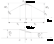
\includegraphics[width=0.5\linewidth]{images/smooth_pos_vel.pdf}
    \caption{Smooth Cartesian trajectory}
    \label{fig:smooth_cartesian_trajectory}
\end{figure}{}

\framebreak

\textcolor{uma_blue_light}{Why do we want to smooth cartesian trajectories?}

To avoid discontinuities in velocities (potentially infinite Cartesian accelerations).

The smooth trajectory is represented by 3 segments:

\begin{enumerate}
    \item The first segment, $t < -\tau$, corresponds to a linear trajectory.
    \item The second segment, $-\tau < t < \tau$, corresponds to the smoothing trajectory. 
    
    In velocity we have a line (both for traslation and orientation), while in position we have a second-order polynomial that assumes a small smoothing error in the smoothing point ($P_1$). 
    
    The more we smooth the trajectory, the higher the error.

    \item The third segment, $\tau < t$, corresponds to a linear trajectory.
\end{enumerate}

If we have a Cartesian path defined by several points, we can move along that way generating a linear Cartesian trajectory between points smoothed in intermediate points (similar to linear trajectories with parabolic blends in the joint space).

\end{frame}

\subsection{Position Smoothing}
\begin{frame}
	\frametitle{Outline} % Table of contents slide, comment this block out to remove it
	\tableofcontents[currentsection,
        currentsubsection] % Throughout your presentation, if you choose to use \section{} and \subsection{} commands, these will automatically be printed on this slide as an overview of your presentation
\end{frame}
\begin{frame}[allowframebreaks]
\frametitle{Position Smoothing}

We must define the smoothing position function between $-\tau$ and $\tau$:
$$
\mathbf{p}(t) = \mathbf{f}(\mathbf{p}_0, \mathbf{p}_1, T_1, T_2, \tau, t^2), \quad t \in [-\tau, \tau], \quad \mathbf{p}(t)\in\mathbb{R}^3
$$
With the boundary conditions for position (left) and velocity (right)
$$
\mathbf{p}(-\tau) = \mathbf{p}_1 - \frac{\tau}{T_1}\Delta \mathbf{p}_1, \quad \quad
\dot{\mathbf{p}}(-\tau) = \frac{\Delta \mathbf{p}_1}{T_1}
$$
$$
\mathbf{p}(\tau) = \mathbf{p}_1 + \frac{\tau}{T_2}\Delta \mathbf{p}_2, \quad \quad
\dot{\mathbf{p}}(\tau) = \frac{\Delta \mathbf{p}_2}{T_2}
$$
\textcolor{uma_pink}{We have 4 conditions (2 for position, and 2 for velocity), but we only need two of them}

The acceleration is constant in the segment $[-\tau, \tau]$ and is defined by the velocities in first and third segments
$$
\ddot{\mathbf{p}} = \frac{\Delta \dot{\mathbf{p}}}{2\tau} = \frac{\dot{\mathbf{p}}(\tau) - \dot{\mathbf{p}}(-\tau)}{2\tau} = \frac{\frac{\Delta \mathbf{p}_2}{T_2} - \frac{\Delta \mathbf{p}_1}{T_1}}{2\tau} = \frac{\Delta \mathbf{p}_2}{2\tau T_2} - \frac{\Delta \mathbf{p}_1}{2\tau T_1}, \quad \ddot{\mathbf{p}}\in\mathbb{R}^3
$$

\framebreak

By integrating the acceleration, we get the smooth trajectory function of the velocity: 
$$
\dot{\mathbf{p}}(t) = \int \ddot{\mathbf{p}}(t) dt = \frac{\Delta \mathbf{p}_2}{2 \tau T_2} t - \frac{\Delta \mathbf{p}_1}{2 \tau T_1} t + \mathbf{C}_1, \quad \dot{\mathbf{p}}(t)\in\mathbb{R}^3, \quad \mathbf{C}_1\in\mathbb{R}^3
$$
Thanks to the first boundary condition for the velocity, we can compute $\mathbf{C}_1$ as:
$$
\mathbf{C}_1 = \frac{\tau \Delta \mathbf{p}_1}{2 \tau T_1} + \frac{\tau \Delta \mathbf{p}_2}{2 \tau T_2}
$$
\textcolor{uma_pink}{Note that if we would have used the second boundary condition, the result would have been the same (symmetric).}

Then
$$
\dot{\mathbf{p}}(t) = \frac{(\tau + t)}{2\tau T_2} \Delta \mathbf{p}_2 + \frac{(\tau - t)}{2\tau T_1} \Delta \mathbf{p}_1
$$

\framebreak

Integrating the velocity expression, we get the smooth position trajectory
$$
\mathbf{p}(t) = \int \dot{\mathbf{p}}(t) dt = \left( \frac{2\tau t + t^2}{4\tau T_2} \right) \Delta \mathbf{p}_2 + \left( \frac{2\tau t - t^2}{4\tau T_1} \right) \Delta \mathbf{p}_1 + \mathbf{C}_2, \quad \mathbf{p}(t)\in\mathbb{R}^3, \quad \mathbf{C}_2\in\mathbb{R}^3
$$
Thanks to the first boundary condition for the position, we can compute $\mathbf{C}_2$ as:
$$
\mathbf{C}_2 = \mathbf{p}_1 + \frac{\tau^2 \Delta \mathbf{p}_2}{4 \tau T_2} - \frac{\tau^2 \Delta \mathbf{p}_1}{4 \tau T_1}
$$
\textcolor{uma_pink}{Note that if we would have used the second boundary condition, the result would have been the same (symmetric).}

Then
\begin{equation}
    \mathbf{p}(t) = \mathbf{p}_1 - \frac{(\tau - t)^2}{4\tau T_1} \Delta \mathbf{p}_1 + \frac{(\tau + t)^2}{4\tau T_2} \Delta \mathbf{p}_2
    \label{eq:p_smooth}
\end{equation}

\end{frame}

\subsection{Orientation Smoothing}
\begin{frame}
	\frametitle{Outline} % Table of contents slide, comment this block out to remove it
	\tableofcontents[currentsection,
        currentsubsection] % Throughout your presentation, if you choose to use \section{} and \subsection{} commands, these will automatically be printed on this slide as an overview of your presentation
\end{frame}
\begin{frame}[allowframebreaks]
\frametitle{Orientation Smoothing}
Now, we have 3 poses. The orientation of each pose is represented by a quaternion $\mathbf{q}_0, \mathbf{q}_1, \mathbf{q}_2$. 

To go from $\mathbf{q}_0$ to $\mathbf{q}_1$, we can get the interpolation quaternion, which has information about a rotation axis $(\mathbf{n}_1)$ and a rotation angle $(\theta_1(\lambda))$ that goes from $\theta_1(0) = 0$ to $\theta_1(1)=\theta_1$. I.e., we use $\lambda$ to modify the rotation angle over time. 

Therefore, we can quantify the rotation change between $\mathbf{q}_0$ and $\mathbf{q}_1$ with $\theta_1$, and the rotation change between $\mathbf{q}_1$ and $\mathbf{q}_2$ with $\theta_2$.

% Hence, we can compute the interpolation quaternions of the first $(t<-\tau)$ and third segments $(\tau<t)$ as:
% \begin{equation}
% \begin{split}
% \mathbf{q}_{01} & =  \mathbf{q}_0 \cdot \mathbf{q}[\theta_1 \lambda(t), \mathbf{n}_1], \quad q[\theta_1, n_1] = q_0^{-1} \cdot q_1\\
% \mathbf{q}_{12} & =  \mathbf{q}_1 \cdot \mathbf{q}[\theta_2 \lambda(t), \mathbf{n}_2], \quad q[\theta_2, n_2] = q_1^{-1} \cdot q_2
% \end{split}
% \end{equation}

% \framebreak
Similarly to what we did with the position, we can smooth the orientation with a second-order polynomial as:
\begin{equation}
    \mathbf{q}(t) = \mathbf{q}_1 \cdot  \underbrace{\mathbf{q} \left[\frac{-(\tau - t)^2}{4\tau T_1} \theta_1, \mathbf{n}_1 \right]}_{\textsf{first smooth interpolation}} \cdot \underbrace{\mathbf{q} \left[ \frac{(\tau + t)^2}{4\tau T_2} \theta_2, \mathbf{n}_2 \right]}_{\textsf{second smooth interpolation}}, \quad t\in[-\tau, \tau]
    \label{eq:q_smooth}
\end{equation}

\framebreak

where 
\begin{equation}
\mathbf{q}_{k_1} = \mathbf{q} \left[\frac{-(\tau - t)^2}{4\tau T_1} \theta_1, \mathbf{n}_1 \right], \quad \quad \mathbf{q}_{k_2} = \mathbf{q} \left[ \frac{(\tau + t)^2}{4\tau T_2} \theta_2, \mathbf{n}_2 \right]
\end{equation}
Can be computed with\\
\begin{minipage}{.45\linewidth}
    \begin{equation}
    \begin{split}
        \mathbf{q}_{01} &= \mathbf{q}_0^{-1} \cdot \mathbf{q}_1\\
        & \theta_{01} = 2 acos(w_{01})\\
        & \mathbf{n}_{01} = \frac{\mathbf{v}_{01}}{sin(\theta_{01}/2 )}
    \end{split}
    \end{equation}
\end{minipage}%
\begin{minipage}{.45\linewidth}
    \begin{equation}
    \begin{split}
        \mathbf{q}_{12} &= \mathbf{q}_1^{-1} \cdot \mathbf{q}_2\\
        & \theta_{12} = 2 acos(w_{12})\\
        & \mathbf{n}_{12} = \frac{\mathbf{v}_{12}}{sin(\theta_{12}/2 )}
    \end{split}
    \end{equation}
\end{minipage}

Therefore
\begin{equation}
    \theta_{k_1} = \frac{-(\tau - t)^2}{4\tau T_1} \theta_{01} \implies \mathbf{q}_{k_1} = \left[cos\left( \frac{\theta_{k_1} }{2}  \right), \, \mathbf{n}_{01} \cdot sin \left(\frac{\theta_{k_1} }{2} \right)\right]
\end{equation}
\begin{equation}
    \theta_{k_2} = \frac{(\tau + t)^2}{4\tau T_1} \theta_{12} \implies \mathbf{q}_{k_2} = \left[cos\left( \frac{\theta_{k_2} }{2}  \right), \, \mathbf{n}_{12} \cdot sin \left(\frac{\theta_{k_2} }{2} \right)\right]
    \label{eq:theta_k2}
\end{equation}


\framebreak
\textcolor{uma_blue_dark}{\textbf{Overall Implementation}}

\begin{algorithm}[H]
	\For{$k = -T: \Delta t: T$}
 	{   
       \If{$k\leq-\tau$}
       {
            $[\mathbf{p_k}, \mathbf{q_k}] = \textsf{qpinter}(P_0, P_1, \frac{k+T}{T}) \quad$ (\ref{eq:p_inter} - \ref{eq:q_inter})
       }
       \ElseIf{$k \geq \tau$}
       {
            $[\mathbf{p_k}, \mathbf{q_k}] = \textsf{qpinter}(P_1, P_2, \frac{k}{T}) \quad$ (\ref{eq:p_inter} - \ref{eq:q_inter})
       }
       \Else
       {
            $\mathbf{p}(k) = \mathbf{p}_1 - \frac{(\tau - k)^2}{4\tau T_1} \Delta \mathbf{p}_1 + \frac{(\tau + k)^2}{4\tau T_2} \Delta \mathbf{p}_2 \quad$ (\ref{eq:p_smooth})\\
            
            $\mathbf{q}(k) = \mathbf{q}_1 \cdot  \mathbf{q}_{k_1}\cdot \mathbf{q}_{k_2}\quad$ (\ref{eq:q_smooth} - \ref{eq:theta_k2})
       }
  	}
\end{algorithm}

\end{frame}


% \section{Optimal Trajectory Planning}
% \begin{frame}
% 	\frametitle{Outline} % Table of contents slide, comment this block out to remove it
% 	\tableofcontents[currentsection,
%         currentsubsection] % Throughout your presentation, if you choose to use \section{} and \subsection{} commands, these will automatically be printed on this slide as an overview of your presentation
% \end{frame}
% \begin{frame}[allowframebreaks]
% \frametitle{Optimal Trajectory Planning}

% ~\cite{vukobratovic1982method}

% \end{frame}


% \begin{frame}[allowframebreaks]
% \frametitle{Dynamic Scaling of Trajectories}

% ~\cite{hollerbach1983dynamic}

% \end{frame}




\begin{frame}[allowframebreaks]
\frametitle{Bibliography}
\printbibliography
\end{frame}

\end{document}